% Hello, world

Since the fall of 2022, I've been teaching intro stats and I've been very particular about my graphs. According to my college ethics professor, the experience of beauty is a human good and statistics is not.\footnote{Shoutout to the late Alfonso G\'{o}mez-Lobo.} That doesn’t provide a good prioritization for developing an intro stats syllabus, but as an instructor, I've at least tried to make my slides and notes a kind of beautiful. Watching a student pinch to zoom on her iPad without a particular graph pixelating or otherwise revealing any defect was a beautiful moment. 

I make all of the figures for my class materials in Python. Working in Python offers the advantage of, well, working in Python. We are able to mix statistical functions from Python in our code, so we gain more precision than is available from anything hand-drawn (whether on pencil and paper or by dragging a cursor). We can also create high quality images in a vector format like PDF or SVG, meaning we can zoom without the image quality degrading. 

It's true that you might achieve the same goals using languages like R or Ti$k$z. Indeed, for probability trees, I still use Ti$k$z. Otherwise, I offer no apology for choosing Python. In this chapter, I include a few common applications that arise in statistics. 


\begin{center}
    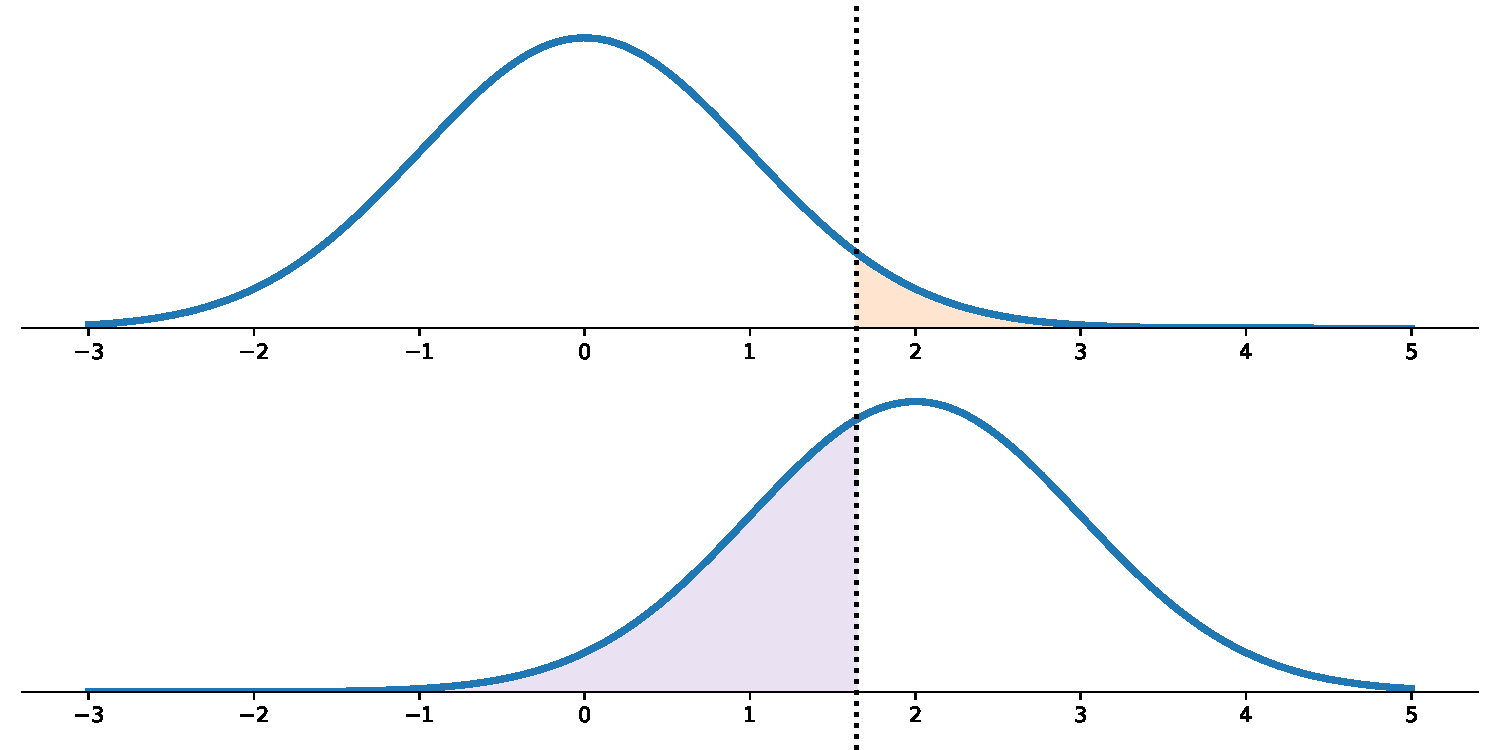
\includegraphics[width = 0.95\textwidth]{figures/specialplots/errors-stacked.pdf}
\end{center}